\documentclass[11pt]{article}
\usepackage[textwidth=18.0cm, textheight=23.0cm, top=2.0cm]{geometry}
\usepackage{pst-all}
\usepackage{amssymb}
\usepackage{tikz}
\usepackage{underscore}\begin{document}
\pagestyle{empty}


ClassName: \underline{\textbf{Class_10.2bp-35}}
\par
BinSize: \underline{\textbf{100 × 100}}
\par
ReduceSize: \underline{\textbf{100 × 100}}
\par
TypeNum: \underline{\textbf{80}}
\par
Num: \underline{\textbf{80}}
\par
OutS: \underline{\textbf{130000}}
\par
InS: \underline{\textbf{122105}}
\par
Rate: \underline{\textbf{0.939}}
\par
UB: \underline{\textbf{13}}
\par
LB0: \underline{\textbf{13}}
\par
LB: \underline{\textbf{13}}
\par
LBWithCut: \underline{\textbf{13}}
\par
NodeCut: \underline{\textbf{0}}
\par
ExtendedNodeCnt: \underline{\textbf{1}}
\par
GenNodeCnt: \underline{\textbf{1}}
\par
PrimalNode: \underline{\textbf{0}}
\par
ColumnCount: \underline{\textbf{13}}
\par
TotalCutCount: \underline{\textbf{0}}
\par
RootCutCount: \underline{\textbf{0}}
\par
LPSolverCnt: \underline{\textbf{1}}
\par
PricingSolverCnt: \underline{\textbf{0}}
\par
BranchAndBoundNum: \underline{\textbf{1}}
\par
isOpt: \underline{\textbf{true}}
\par
TimeOnInitSolution: \underline{\textbf{600.000 s}}
\par
TimeOnPrimal: \underline{\textbf{0.000 s}}
\par
TimeOnPricing: \underline{\textbf{0.000 s}}
\par
TimeOnRmp: \underline{\textbf{0.078 s}}
\par
TotalTime: \underline{\textbf{600.328 s}}
\par
\newpage


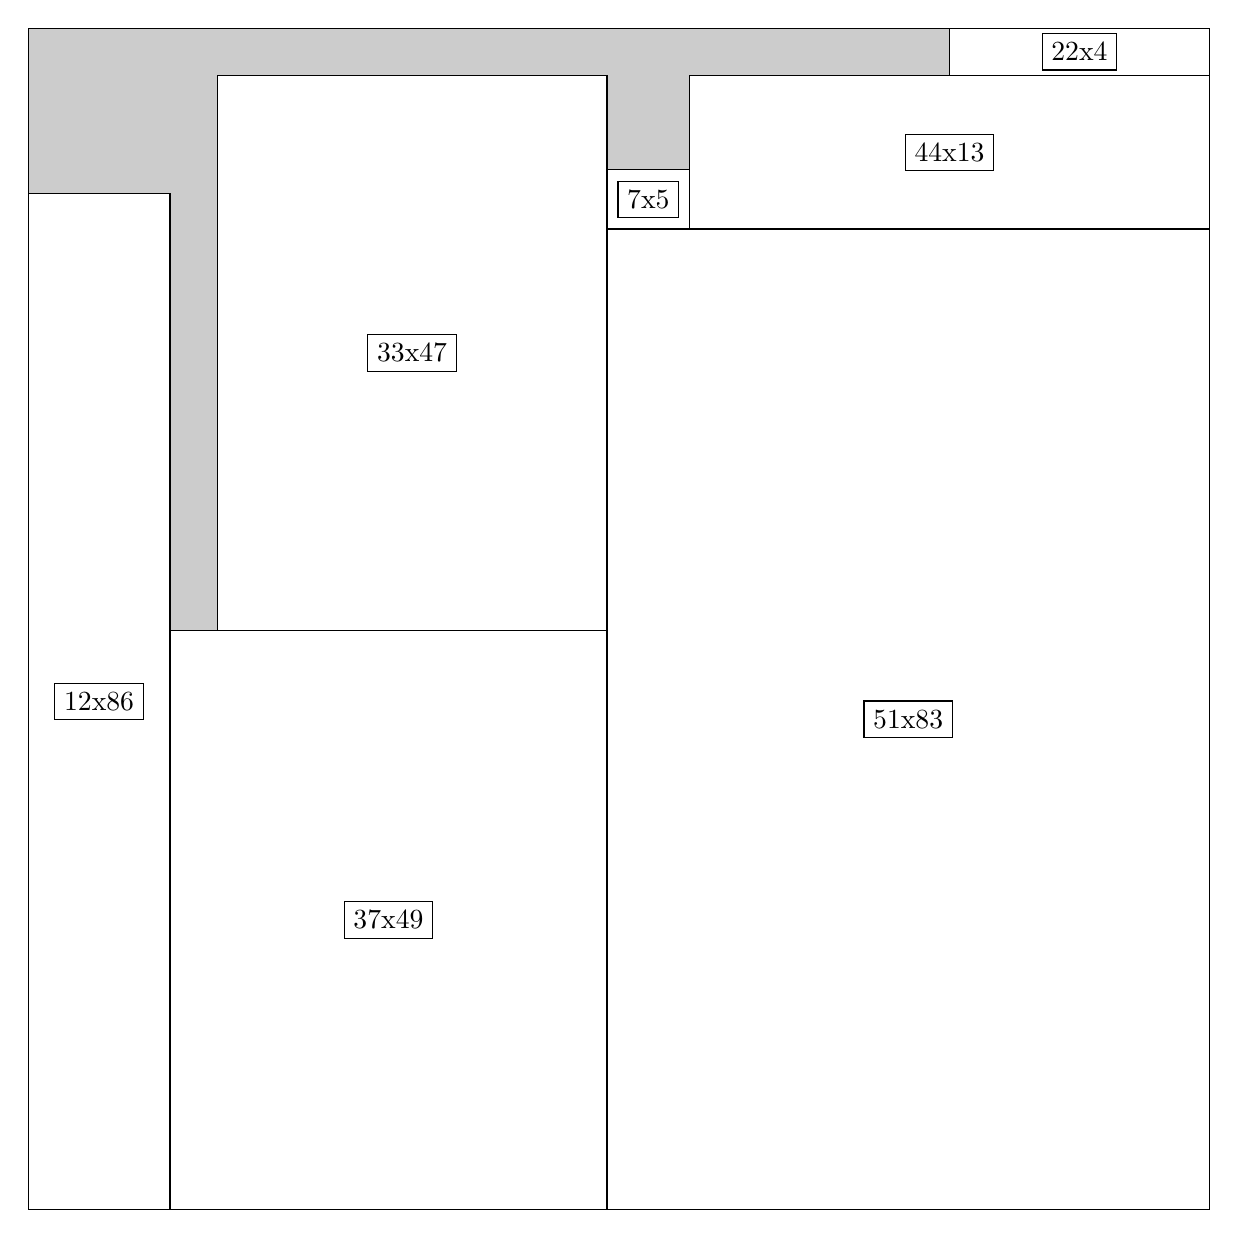
\begin{tikzpicture}[shorten >=1pt,scale=1.0,every node/.style={scale=1.0},->]
\tikzstyle{vertex}=[circle,fill=black!25,minimum size=14pt,inner sep=0pt]
\filldraw[fill=gray!40!white, draw=black] (0,0) rectangle (15.0,15.0);
\foreach \name/\x/\y/\w/\h in {51x83/7.35/0.0/7.6499999999999995/12.45,44x13/8.4/12.45/6.6/1.95,7x5/7.35/12.45/1.05/0.75,22x4/11.7/14.399999999999999/3.3/0.6,37x49/1.7999999999999998/0.0/5.55/7.35,33x47/2.4/7.35/4.95/7.05,12x86/0.0/0.0/1.7999999999999998/12.9}
\filldraw[fill=white!40!white, draw=black] (\x,\y) rectangle node[draw] (\name) {\name} ++(\w,\h);
\end{tikzpicture}


w =51 , h =83 , x =49 , y =0 , v =4233
\par
w =44 , h =13 , x =56 , y =83 , v =572
\par
w =7 , h =5 , x =49 , y =83 , v =35
\par
w =22 , h =4 , x =78 , y =96 , v =88
\par
w =37 , h =49 , x =12 , y =0 , v =1813
\par
w =33 , h =47 , x =16 , y =49 , v =1551
\par
w =12 , h =86 , x =0 , y =0 , v =1032
\par
\newpage


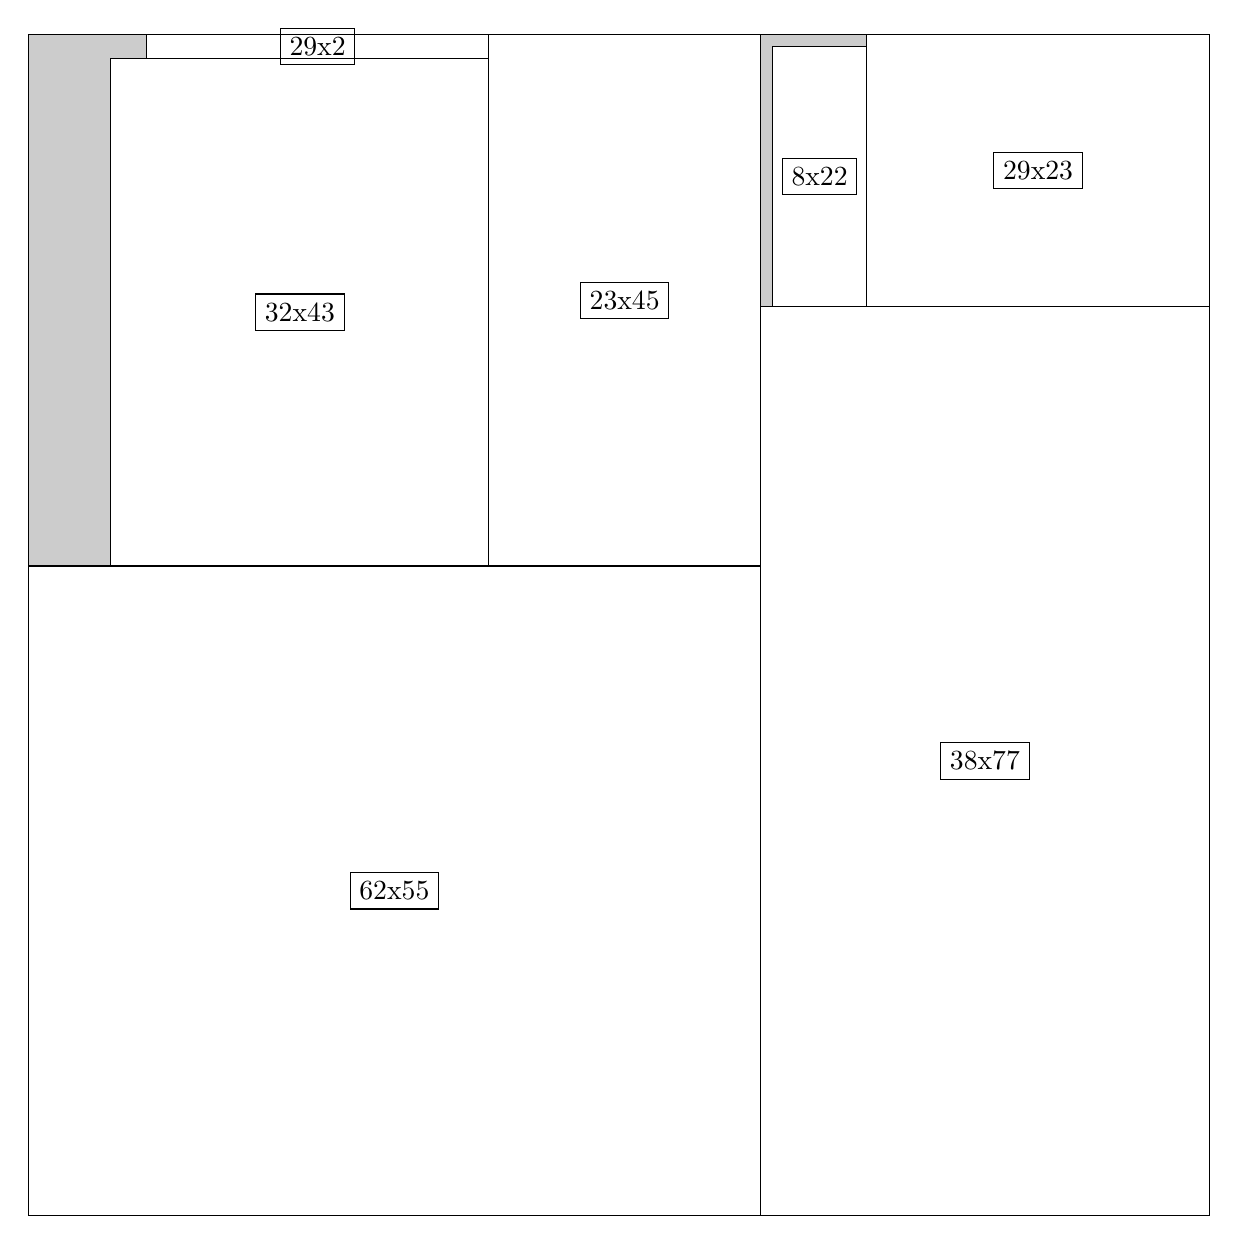
\begin{tikzpicture}[shorten >=1pt,scale=1.0,every node/.style={scale=1.0},->]
\tikzstyle{vertex}=[circle,fill=black!25,minimum size=14pt,inner sep=0pt]
\filldraw[fill=gray!40!white, draw=black] (0,0) rectangle (15.0,15.0);
\foreach \name/\x/\y/\w/\h in {38x77/9.299999999999999/0.0/5.7/11.549999999999999,29x23/10.65/11.549999999999999/4.35/3.4499999999999997,8x22/9.45/11.549999999999999/1.2/3.3,62x55/0.0/0.0/9.299999999999999/8.25,23x45/5.85/8.25/3.4499999999999997/6.75,32x43/1.05/8.25/4.8/6.45,29x2/1.5/14.7/4.35/0.3}
\filldraw[fill=white!40!white, draw=black] (\x,\y) rectangle node[draw] (\name) {\name} ++(\w,\h);
\end{tikzpicture}


w =38 , h =77 , x =62 , y =0 , v =2926
\par
w =29 , h =23 , x =71 , y =77 , v =667
\par
w =8 , h =22 , x =63 , y =77 , v =176
\par
w =62 , h =55 , x =0 , y =0 , v =3410
\par
w =23 , h =45 , x =39 , y =55 , v =1035
\par
w =32 , h =43 , x =7 , y =55 , v =1376
\par
w =29 , h =2 , x =10 , y =98 , v =58
\par
\newpage


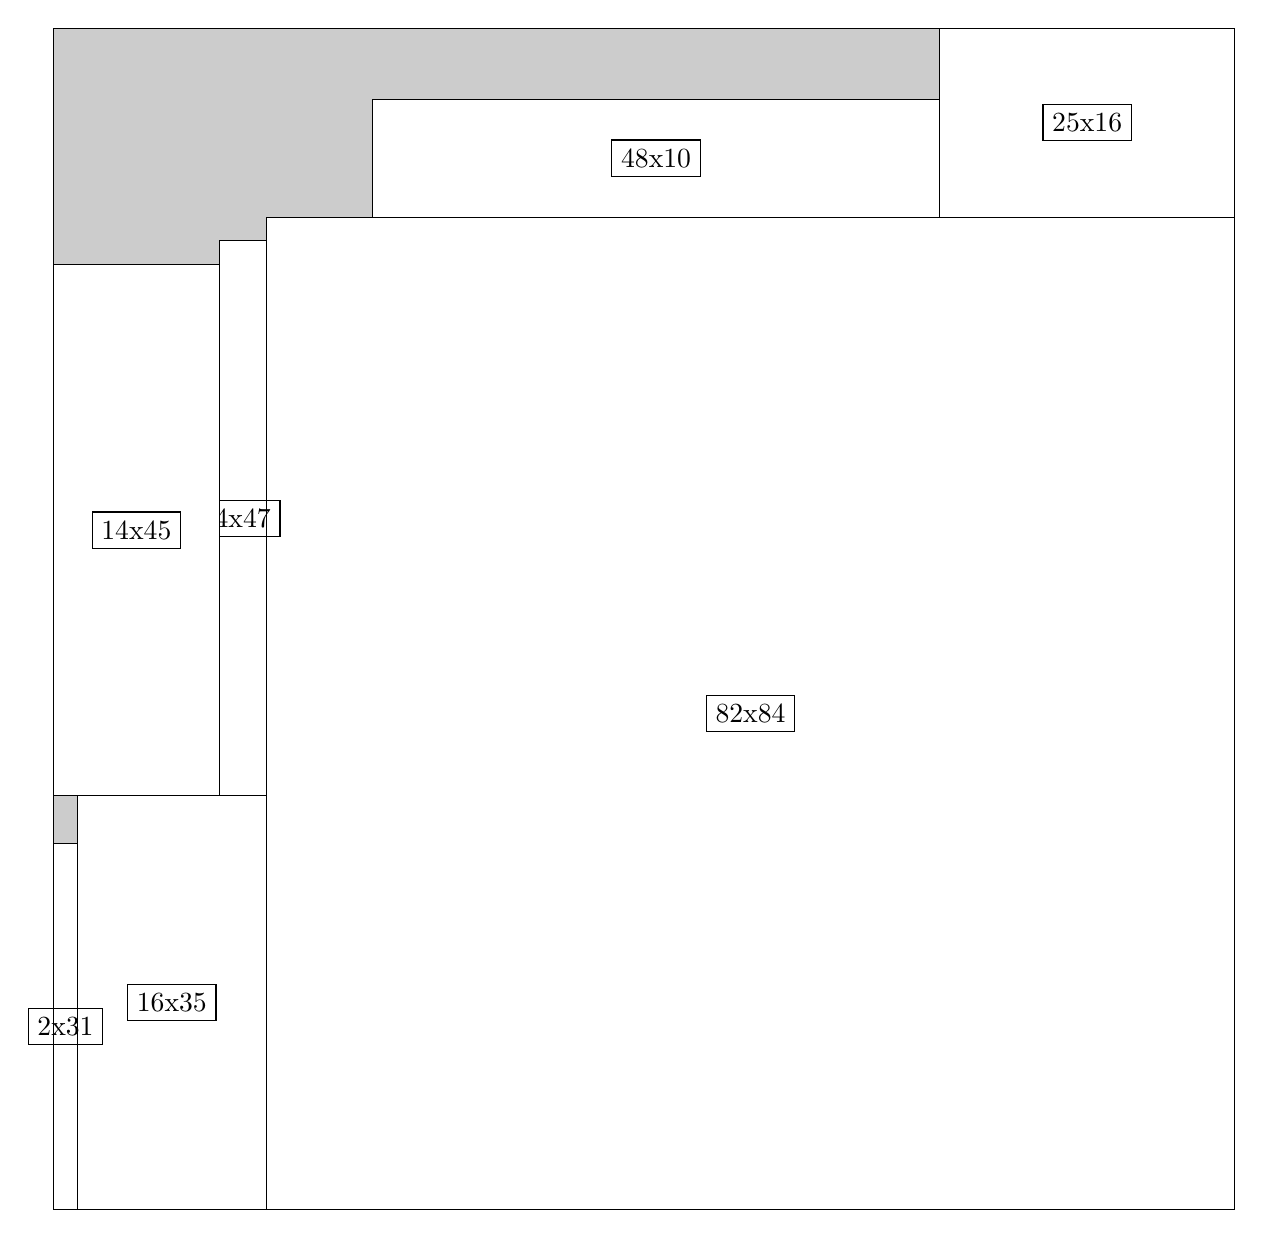
\begin{tikzpicture}[shorten >=1pt,scale=1.0,every node/.style={scale=1.0},->]
\tikzstyle{vertex}=[circle,fill=black!25,minimum size=14pt,inner sep=0pt]
\filldraw[fill=gray!40!white, draw=black] (0,0) rectangle (15.0,15.0);
\foreach \name/\x/\y/\w/\h in {82x84/2.6999999999999997/0.0/12.299999999999999/12.6,25x16/11.25/12.6/3.75/2.4,48x10/4.05/12.6/7.199999999999999/1.5,16x35/0.3/0.0/2.4/5.25,2x31/0.0/0.0/0.3/4.6499999999999995,4x47/2.1/5.25/0.6/7.05,14x45/0.0/5.25/2.1/6.75}
\filldraw[fill=white!40!white, draw=black] (\x,\y) rectangle node[draw] (\name) {\name} ++(\w,\h);
\end{tikzpicture}


w =82 , h =84 , x =18 , y =0 , v =6888
\par
w =25 , h =16 , x =75 , y =84 , v =400
\par
w =48 , h =10 , x =27 , y =84 , v =480
\par
w =16 , h =35 , x =2 , y =0 , v =560
\par
w =2 , h =31 , x =0 , y =0 , v =62
\par
w =4 , h =47 , x =14 , y =35 , v =188
\par
w =14 , h =45 , x =0 , y =35 , v =630
\par
\newpage


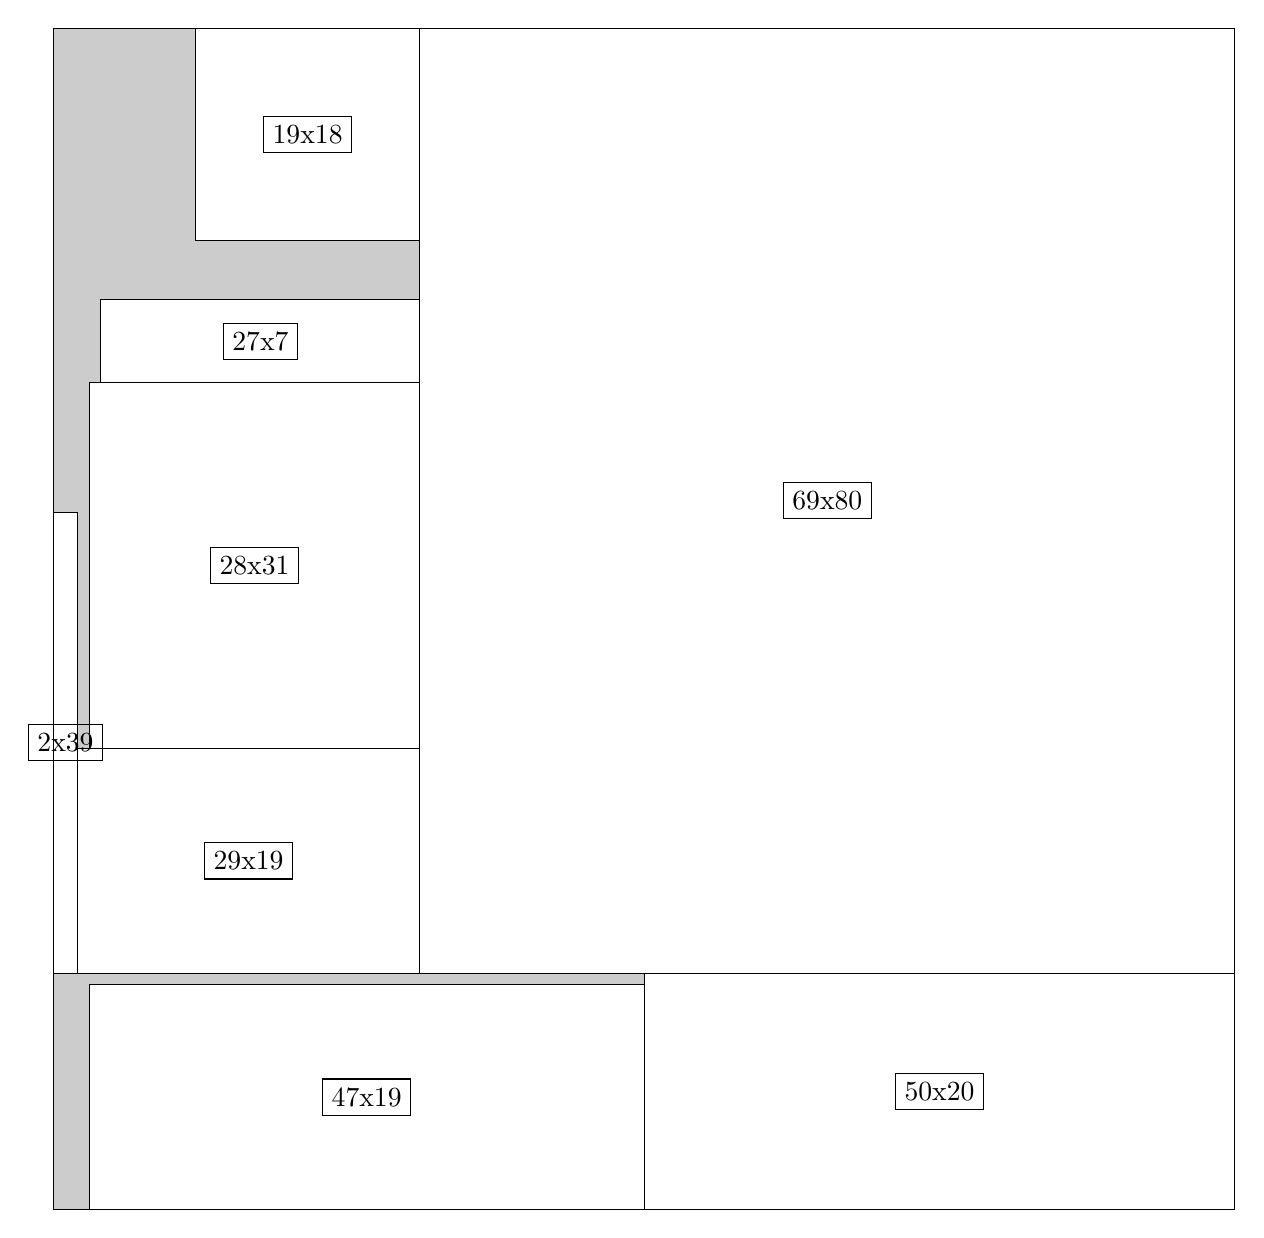
\begin{tikzpicture}[shorten >=1pt,scale=1.0,every node/.style={scale=1.0},->]
\tikzstyle{vertex}=[circle,fill=black!25,minimum size=14pt,inner sep=0pt]
\filldraw[fill=gray!40!white, draw=black] (0,0) rectangle (15.0,15.0);
\foreach \name/\x/\y/\w/\h in {50x20/7.5/0.0/7.5/3.0,47x19/0.44999999999999996/0.0/7.05/2.85,69x80/4.6499999999999995/3.0/10.35/12.0,29x19/0.3/3.0/4.35/2.85,28x31/0.44999999999999996/5.85/4.2/4.6499999999999995,27x7/0.6/10.5/4.05/1.05,19x18/1.7999999999999998/12.299999999999999/2.85/2.6999999999999997,2x39/0.0/3.0/0.3/5.85}
\filldraw[fill=white!40!white, draw=black] (\x,\y) rectangle node[draw] (\name) {\name} ++(\w,\h);
\end{tikzpicture}


w =50 , h =20 , x =50 , y =0 , v =1000
\par
w =47 , h =19 , x =3 , y =0 , v =893
\par
w =69 , h =80 , x =31 , y =20 , v =5520
\par
w =29 , h =19 , x =2 , y =20 , v =551
\par
w =28 , h =31 , x =3 , y =39 , v =868
\par
w =27 , h =7 , x =4 , y =70 , v =189
\par
w =19 , h =18 , x =12 , y =82 , v =342
\par
w =2 , h =39 , x =0 , y =20 , v =78
\par
\newpage


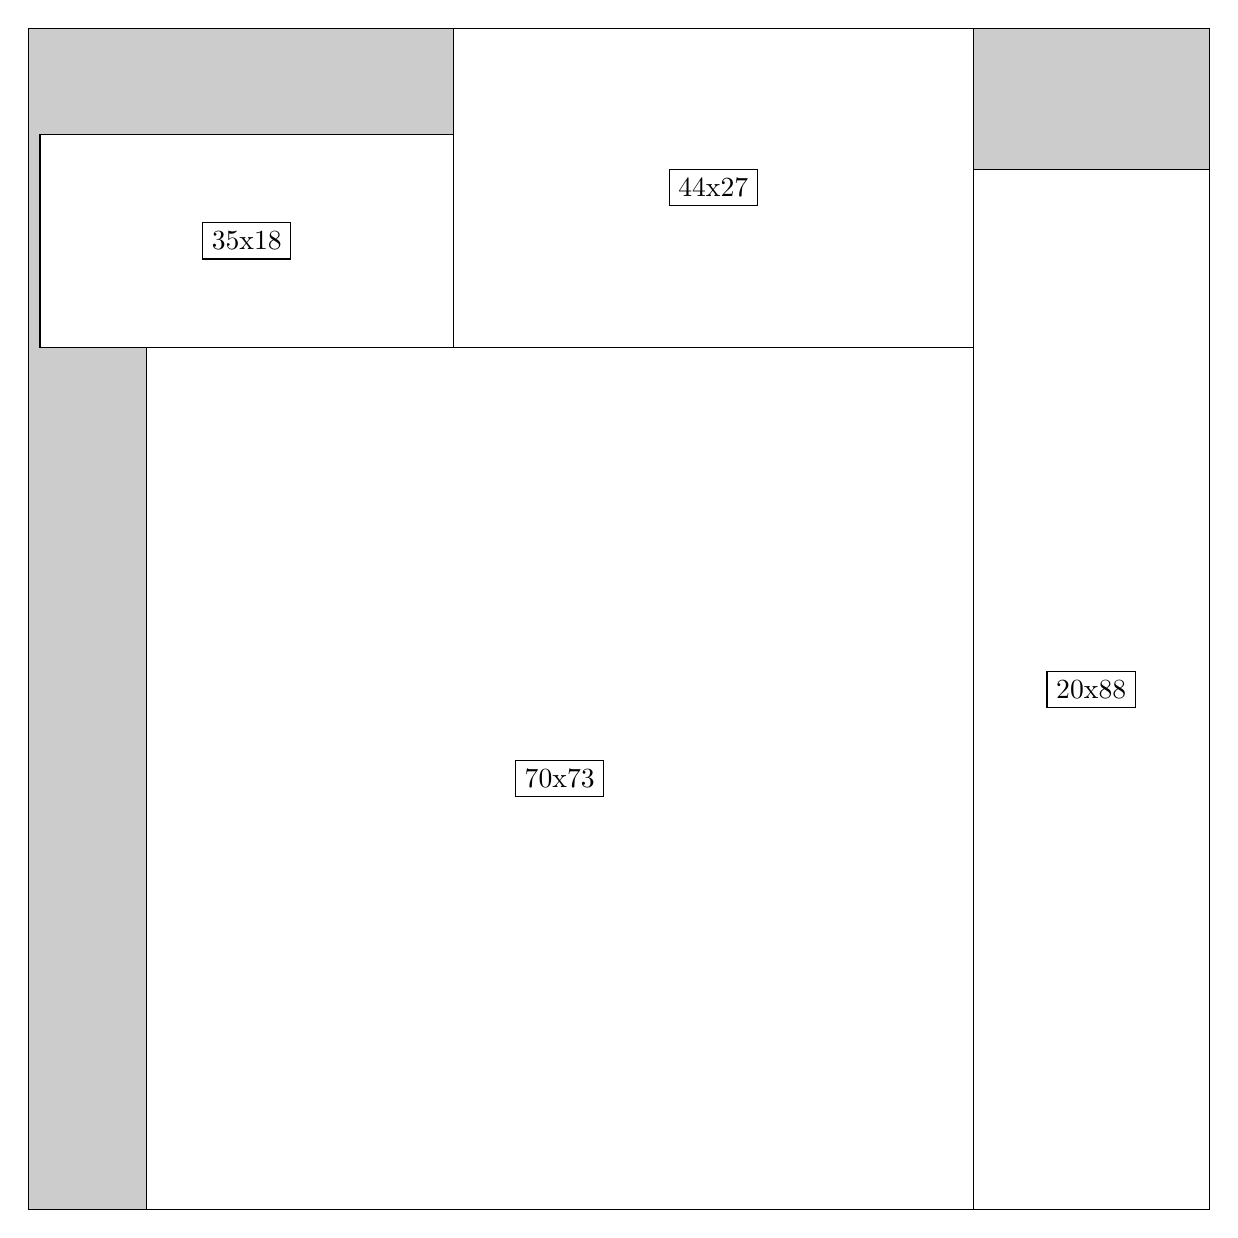
\begin{tikzpicture}[shorten >=1pt,scale=1.0,every node/.style={scale=1.0},->]
\tikzstyle{vertex}=[circle,fill=black!25,minimum size=14pt,inner sep=0pt]
\filldraw[fill=gray!40!white, draw=black] (0,0) rectangle (15.0,15.0);
\foreach \name/\x/\y/\w/\h in {20x88/12.0/0.0/3.0/13.2,70x73/1.5/0.0/10.5/10.95,44x27/5.3999999999999995/10.95/6.6/4.05,35x18/0.15/10.95/5.25/2.6999999999999997}
\filldraw[fill=white!40!white, draw=black] (\x,\y) rectangle node[draw] (\name) {\name} ++(\w,\h);
\end{tikzpicture}


w =20 , h =88 , x =80 , y =0 , v =1760
\par
w =70 , h =73 , x =10 , y =0 , v =5110
\par
w =44 , h =27 , x =36 , y =73 , v =1188
\par
w =35 , h =18 , x =1 , y =73 , v =630
\par
\newpage


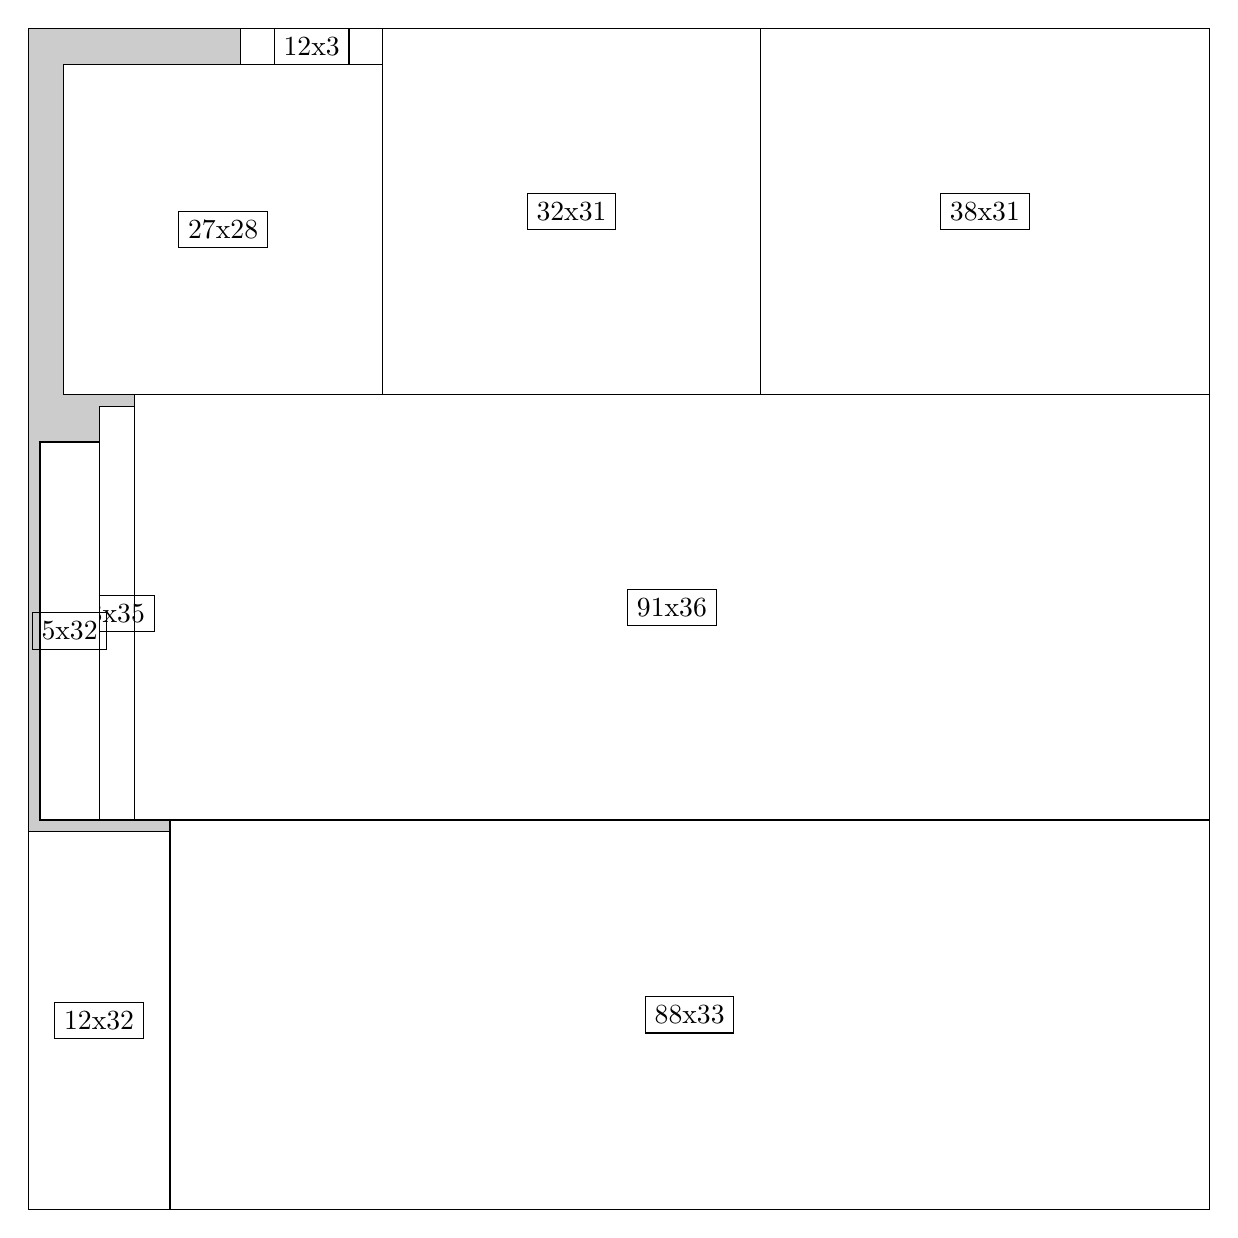
\begin{tikzpicture}[shorten >=1pt,scale=1.0,every node/.style={scale=1.0},->]
\tikzstyle{vertex}=[circle,fill=black!25,minimum size=14pt,inner sep=0pt]
\filldraw[fill=gray!40!white, draw=black] (0,0) rectangle (15.0,15.0);
\foreach \name/\x/\y/\w/\h in {88x33/1.7999999999999998/0.0/13.2/4.95,12x32/0.0/0.0/1.7999999999999998/4.8,91x36/1.3499999999999999/4.95/13.65/5.3999999999999995,3x35/0.8999999999999999/4.95/0.44999999999999996/5.25,5x32/0.15/4.95/0.75/4.8,38x31/9.299999999999999/10.35/5.7/4.6499999999999995,32x31/4.5/10.35/4.8/4.6499999999999995,27x28/0.44999999999999996/10.35/4.05/4.2,12x3/2.6999999999999997/14.549999999999999/1.7999999999999998/0.44999999999999996}
\filldraw[fill=white!40!white, draw=black] (\x,\y) rectangle node[draw] (\name) {\name} ++(\w,\h);
\end{tikzpicture}


w =88 , h =33 , x =12 , y =0 , v =2904
\par
w =12 , h =32 , x =0 , y =0 , v =384
\par
w =91 , h =36 , x =9 , y =33 , v =3276
\par
w =3 , h =35 , x =6 , y =33 , v =105
\par
w =5 , h =32 , x =1 , y =33 , v =160
\par
w =38 , h =31 , x =62 , y =69 , v =1178
\par
w =32 , h =31 , x =30 , y =69 , v =992
\par
w =27 , h =28 , x =3 , y =69 , v =756
\par
w =12 , h =3 , x =18 , y =97 , v =36
\par
\newpage


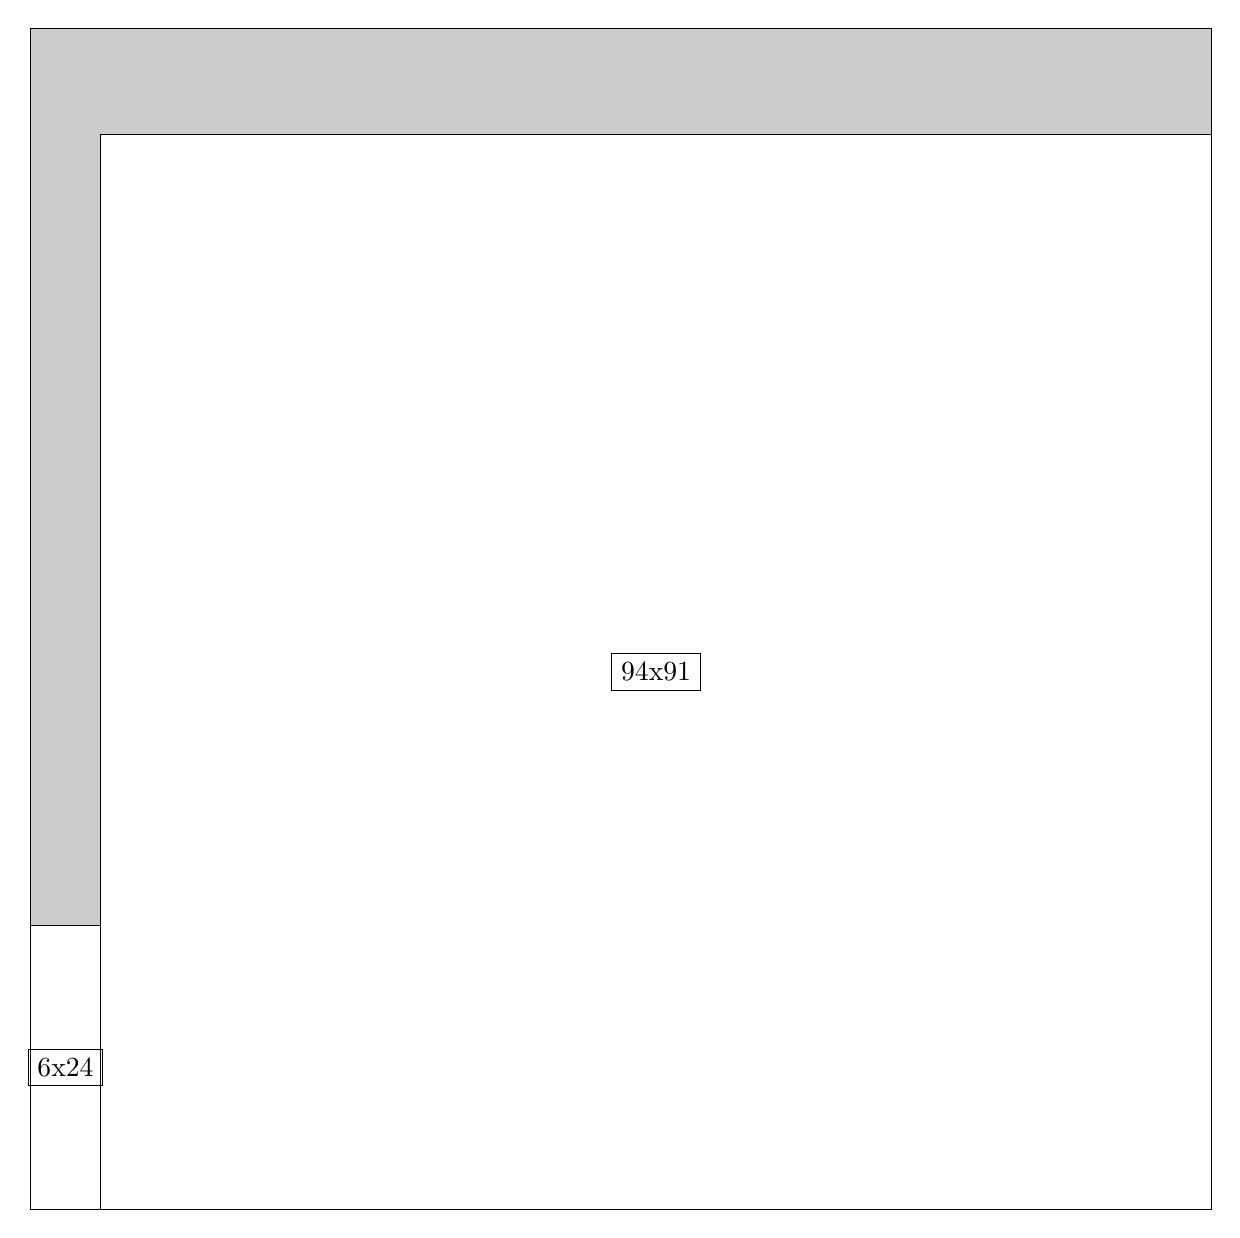
\begin{tikzpicture}[shorten >=1pt,scale=1.0,every node/.style={scale=1.0},->]
\tikzstyle{vertex}=[circle,fill=black!25,minimum size=14pt,inner sep=0pt]
\filldraw[fill=gray!40!white, draw=black] (0,0) rectangle (15.0,15.0);
\foreach \name/\x/\y/\w/\h in {94x91/0.8999999999999999/0.0/14.1/13.65,6x24/0.0/0.0/0.8999999999999999/3.5999999999999996}
\filldraw[fill=white!40!white, draw=black] (\x,\y) rectangle node[draw] (\name) {\name} ++(\w,\h);
\end{tikzpicture}


w =94 , h =91 , x =6 , y =0 , v =8554
\par
w =6 , h =24 , x =0 , y =0 , v =144
\par
\newpage


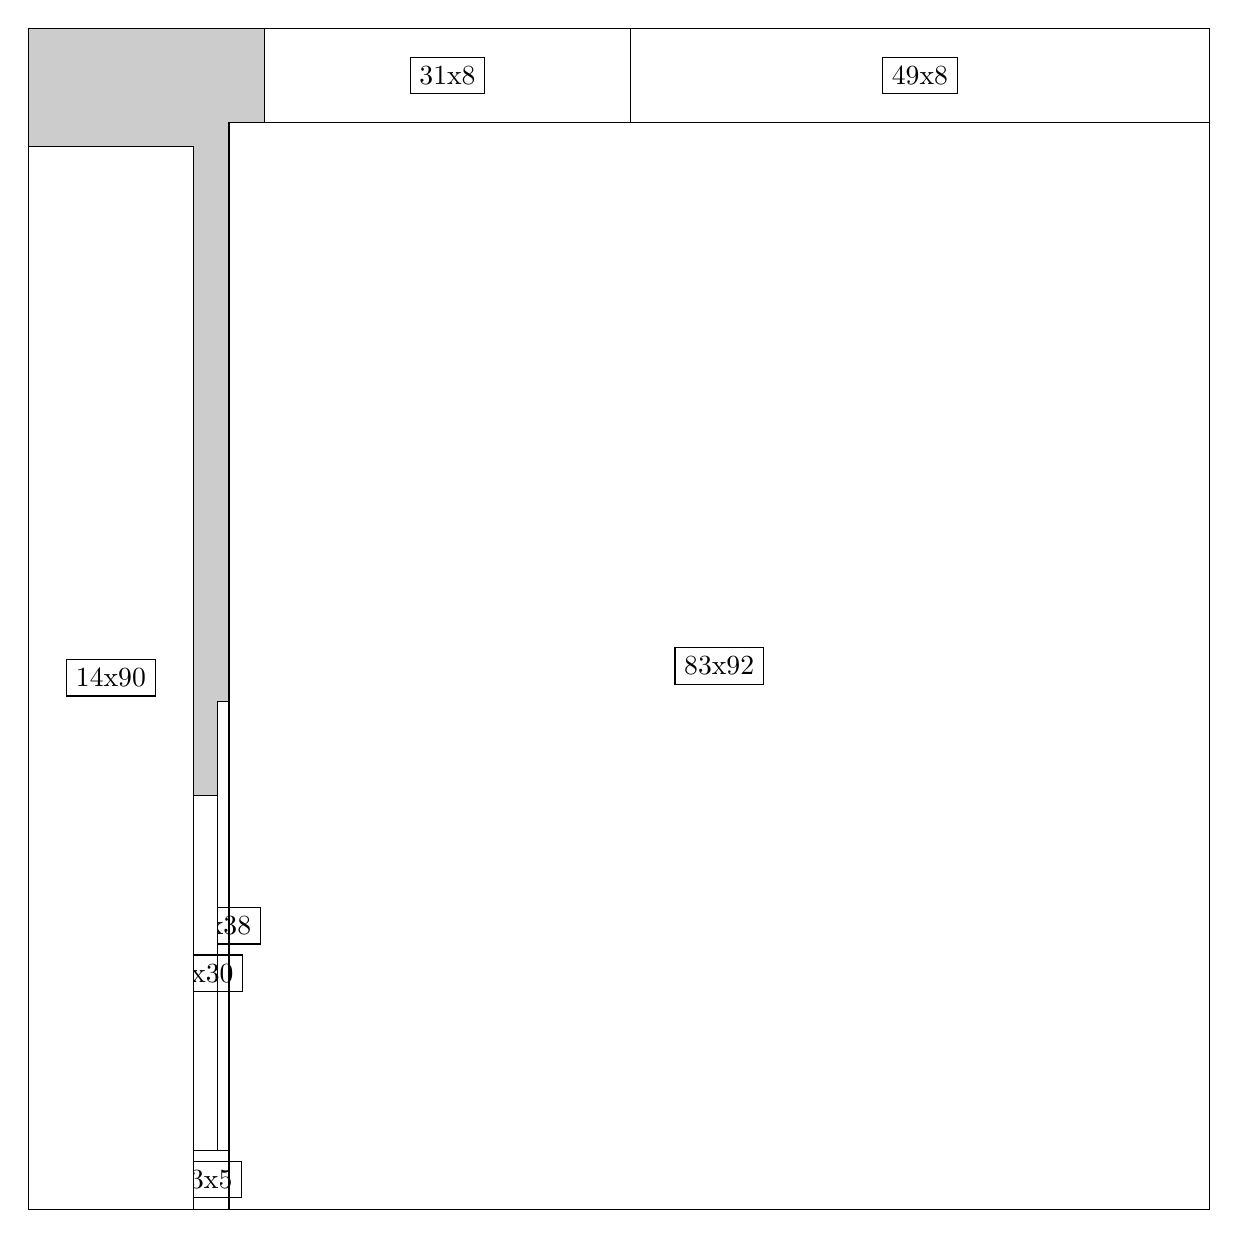
\begin{tikzpicture}[shorten >=1pt,scale=1.0,every node/.style={scale=1.0},->]
\tikzstyle{vertex}=[circle,fill=black!25,minimum size=14pt,inner sep=0pt]
\filldraw[fill=gray!40!white, draw=black] (0,0) rectangle (15.0,15.0);
\foreach \name/\x/\y/\w/\h in {83x92/2.55/0.0/12.45/13.799999999999999,3x5/2.1/0.0/0.44999999999999996/0.75,1x38/2.4/0.75/0.15/5.7,2x30/2.1/0.75/0.3/4.5,49x8/7.6499999999999995/13.799999999999999/7.35/1.2,31x8/3.0/13.799999999999999/4.6499999999999995/1.2,14x90/0.0/0.0/2.1/13.5}
\filldraw[fill=white!40!white, draw=black] (\x,\y) rectangle node[draw] (\name) {\name} ++(\w,\h);
\end{tikzpicture}


w =83 , h =92 , x =17 , y =0 , v =7636
\par
w =3 , h =5 , x =14 , y =0 , v =15
\par
w =1 , h =38 , x =16 , y =5 , v =38
\par
w =2 , h =30 , x =14 , y =5 , v =60
\par
w =49 , h =8 , x =51 , y =92 , v =392
\par
w =31 , h =8 , x =20 , y =92 , v =248
\par
w =14 , h =90 , x =0 , y =0 , v =1260
\par
\newpage


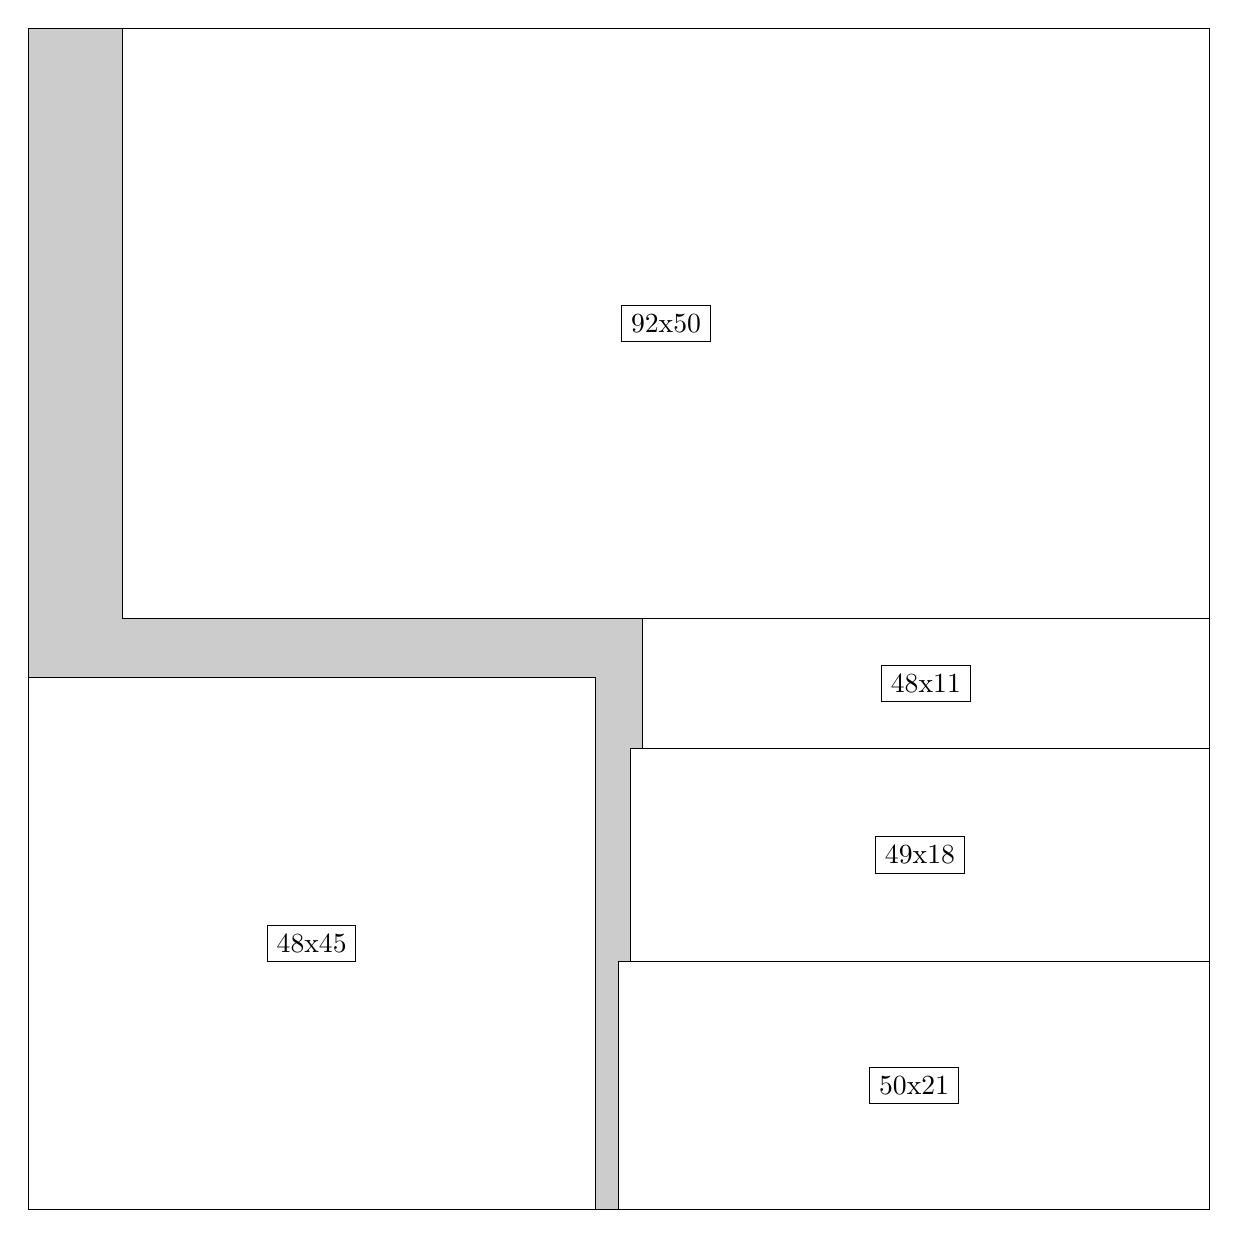
\begin{tikzpicture}[shorten >=1pt,scale=1.0,every node/.style={scale=1.0},->]
\tikzstyle{vertex}=[circle,fill=black!25,minimum size=14pt,inner sep=0pt]
\filldraw[fill=gray!40!white, draw=black] (0,0) rectangle (15.0,15.0);
\foreach \name/\x/\y/\w/\h in {50x21/7.5/0.0/7.5/3.15,49x18/7.6499999999999995/3.15/7.35/2.6999999999999997,48x11/7.8/5.85/7.199999999999999/1.65,48x45/0.0/0.0/7.199999999999999/6.75,92x50/1.2/7.5/13.799999999999999/7.5}
\filldraw[fill=white!40!white, draw=black] (\x,\y) rectangle node[draw] (\name) {\name} ++(\w,\h);
\end{tikzpicture}


w =50 , h =21 , x =50 , y =0 , v =1050
\par
w =49 , h =18 , x =51 , y =21 , v =882
\par
w =48 , h =11 , x =52 , y =39 , v =528
\par
w =48 , h =45 , x =0 , y =0 , v =2160
\par
w =92 , h =50 , x =8 , y =50 , v =4600
\par
\newpage


\begin{tikzpicture}[shorten >=1pt,scale=1.0,every node/.style={scale=1.0},->]
\tikzstyle{vertex}=[circle,fill=black!25,minimum size=14pt,inner sep=0pt]
\filldraw[fill=gray!40!white, draw=black] (0,0) rectangle (15.0,15.0);
\foreach \name/\x/\y/\w/\h in {22x67/11.7/0.0/3.3/10.049999999999999,22x33/11.7/10.049999999999999/3.3/4.95,78x61/0.0/0.0/11.7/9.15,49x39/4.35/9.15/7.35/5.85,29x36/0.0/9.15/4.35/5.3999999999999995}
\filldraw[fill=white!40!white, draw=black] (\x,\y) rectangle node[draw] (\name) {\name} ++(\w,\h);
\end{tikzpicture}


w =22 , h =67 , x =78 , y =0 , v =1474
\par
w =22 , h =33 , x =78 , y =67 , v =726
\par
w =78 , h =61 , x =0 , y =0 , v =4758
\par
w =49 , h =39 , x =29 , y =61 , v =1911
\par
w =29 , h =36 , x =0 , y =61 , v =1044
\par
\newpage


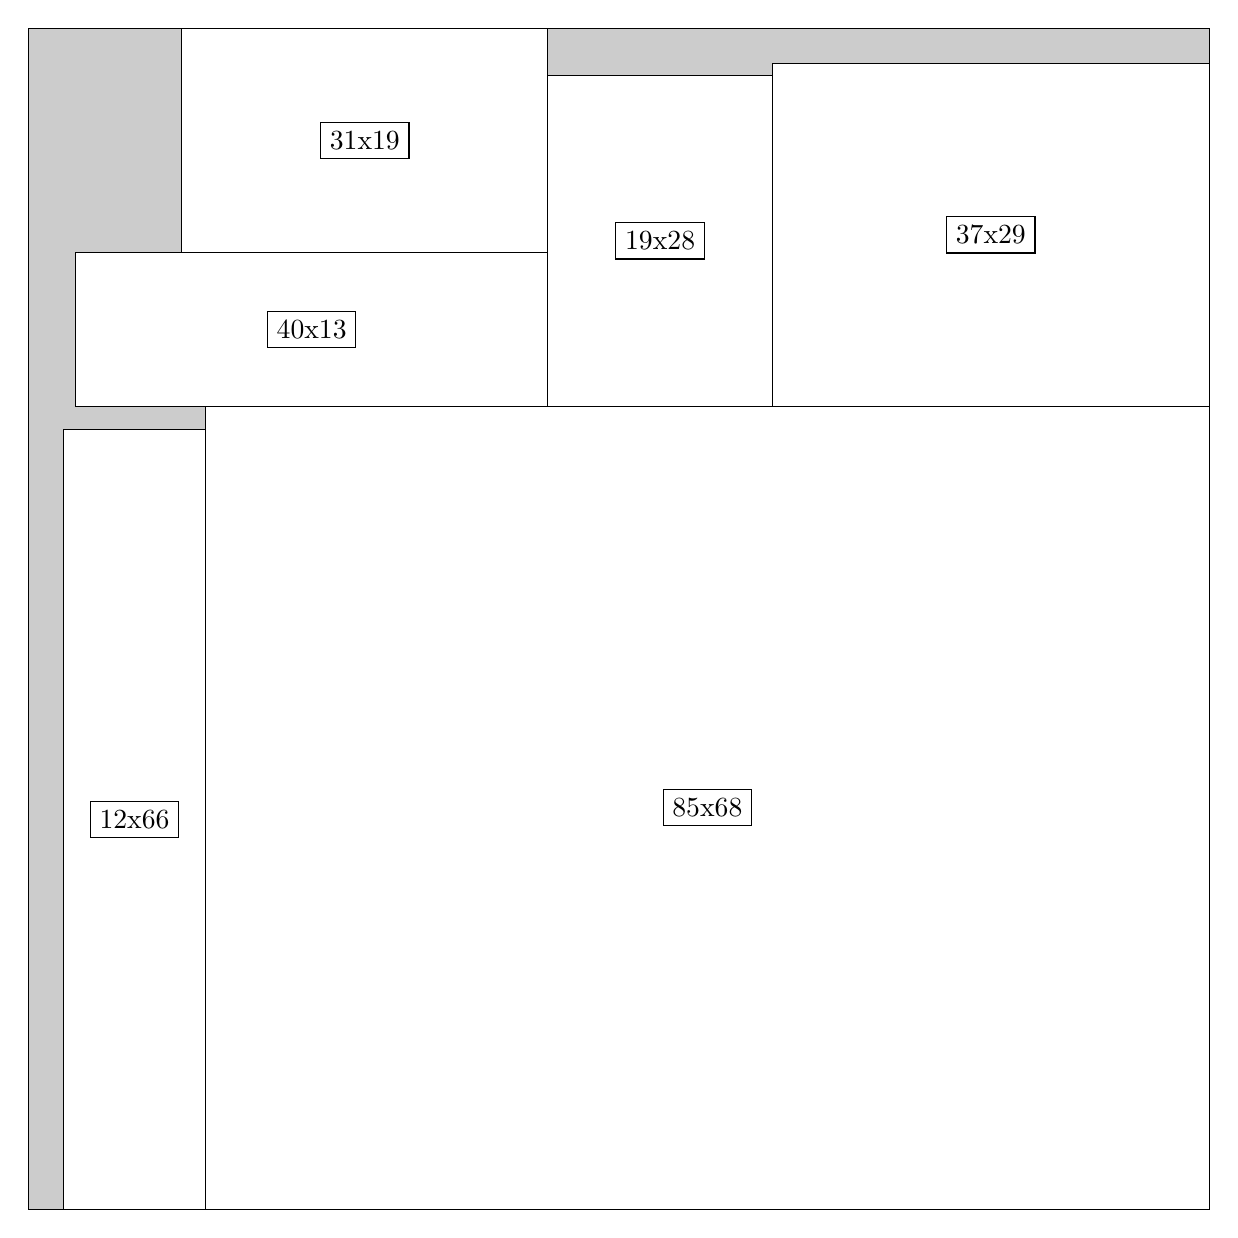
\begin{tikzpicture}[shorten >=1pt,scale=1.0,every node/.style={scale=1.0},->]
\tikzstyle{vertex}=[circle,fill=black!25,minimum size=14pt,inner sep=0pt]
\filldraw[fill=gray!40!white, draw=black] (0,0) rectangle (15.0,15.0);
\foreach \name/\x/\y/\w/\h in {85x68/2.25/0.0/12.75/10.2,12x66/0.44999999999999996/0.0/1.7999999999999998/9.9,37x29/9.45/10.2/5.55/4.35,19x28/6.6/10.2/2.85/4.2,40x13/0.6/10.2/6.0/1.95,31x19/1.95/12.15/4.6499999999999995/2.85}
\filldraw[fill=white!40!white, draw=black] (\x,\y) rectangle node[draw] (\name) {\name} ++(\w,\h);
\end{tikzpicture}


w =85 , h =68 , x =15 , y =0 , v =5780
\par
w =12 , h =66 , x =3 , y =0 , v =792
\par
w =37 , h =29 , x =63 , y =68 , v =1073
\par
w =19 , h =28 , x =44 , y =68 , v =532
\par
w =40 , h =13 , x =4 , y =68 , v =520
\par
w =31 , h =19 , x =13 , y =81 , v =589
\par
\newpage


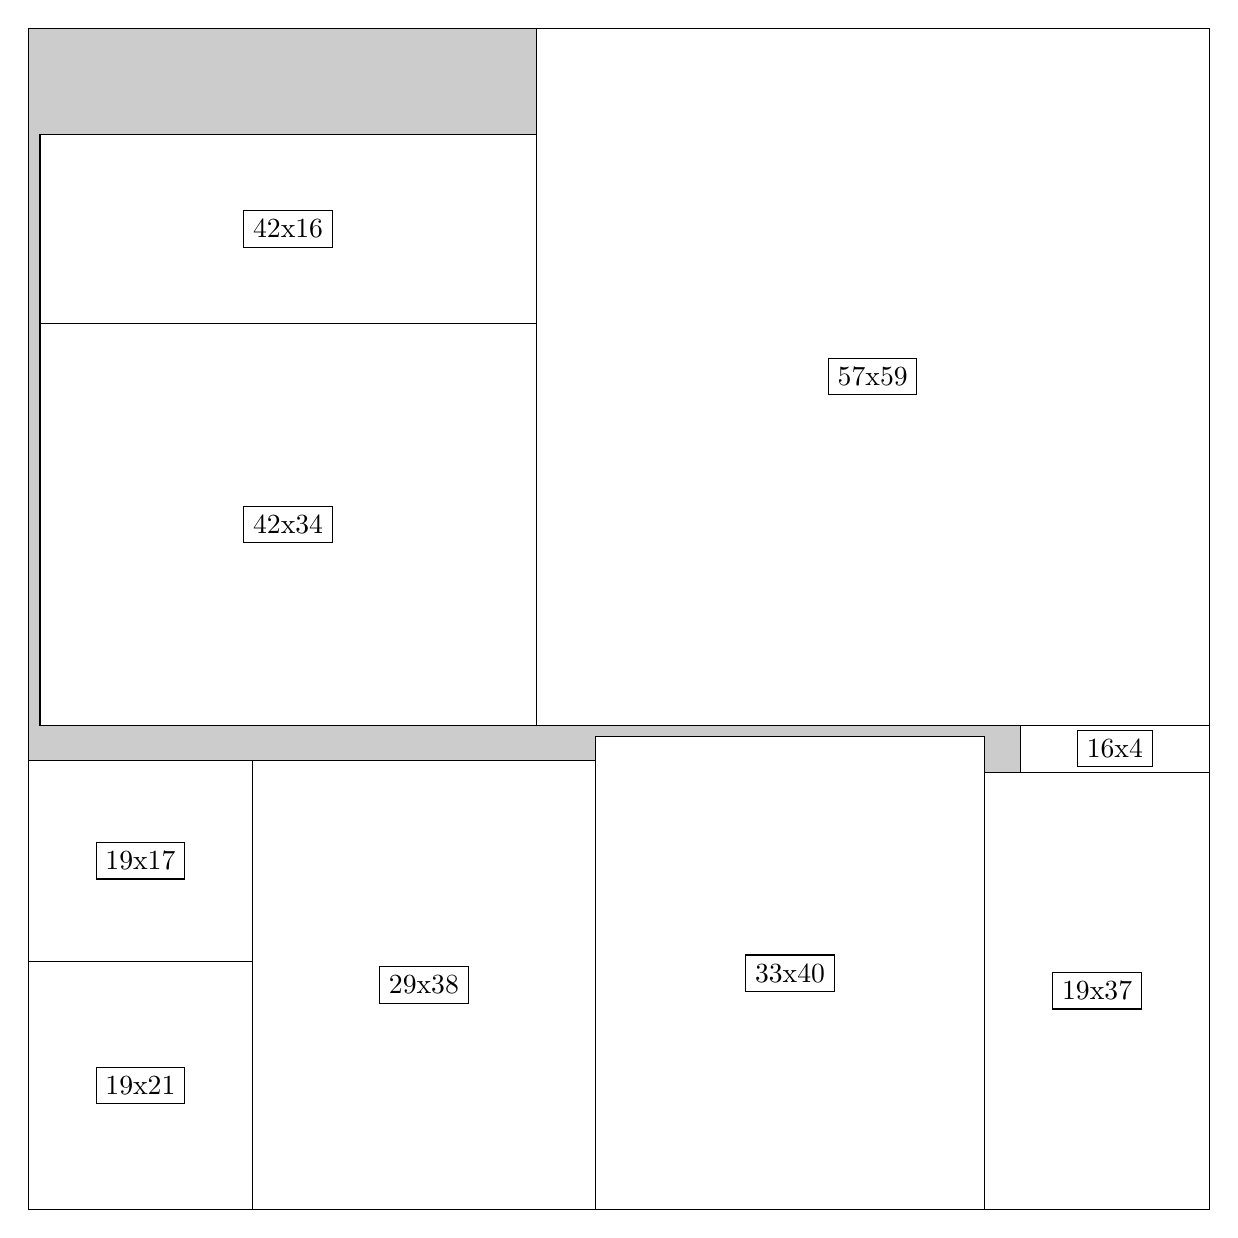
\begin{tikzpicture}[shorten >=1pt,scale=1.0,every node/.style={scale=1.0},->]
\tikzstyle{vertex}=[circle,fill=black!25,minimum size=14pt,inner sep=0pt]
\filldraw[fill=gray!40!white, draw=black] (0,0) rectangle (15.0,15.0);
\foreach \name/\x/\y/\w/\h in {19x37/12.15/0.0/2.85/5.55,16x4/12.6/5.55/2.4/0.6,33x40/7.199999999999999/0.0/4.95/6.0,29x38/2.85/0.0/4.35/5.7,19x21/0.0/0.0/2.85/3.15,19x17/0.0/3.15/2.85/2.55,57x59/6.45/6.1499999999999995/8.549999999999999/8.85,42x34/0.15/6.1499999999999995/6.3/5.1,42x16/0.15/11.25/6.3/2.4}
\filldraw[fill=white!40!white, draw=black] (\x,\y) rectangle node[draw] (\name) {\name} ++(\w,\h);
\end{tikzpicture}


w =19 , h =37 , x =81 , y =0 , v =703
\par
w =16 , h =4 , x =84 , y =37 , v =64
\par
w =33 , h =40 , x =48 , y =0 , v =1320
\par
w =29 , h =38 , x =19 , y =0 , v =1102
\par
w =19 , h =21 , x =0 , y =0 , v =399
\par
w =19 , h =17 , x =0 , y =21 , v =323
\par
w =57 , h =59 , x =43 , y =41 , v =3363
\par
w =42 , h =34 , x =1 , y =41 , v =1428
\par
w =42 , h =16 , x =1 , y =75 , v =672
\par
\newpage


\begin{tikzpicture}[shorten >=1pt,scale=1.0,every node/.style={scale=1.0},->]
\tikzstyle{vertex}=[circle,fill=black!25,minimum size=14pt,inner sep=0pt]
\filldraw[fill=gray!40!white, draw=black] (0,0) rectangle (15.0,15.0);
\foreach \name/\x/\y/\w/\h in {91x41/1.3499999999999999/0.0/13.65/6.1499999999999995,9x39/0.0/0.0/1.3499999999999999/5.85,87x59/1.95/6.1499999999999995/13.049999999999999/8.85,13x50/0.0/6.1499999999999995/1.95/7.5}
\filldraw[fill=white!40!white, draw=black] (\x,\y) rectangle node[draw] (\name) {\name} ++(\w,\h);
\end{tikzpicture}


w =91 , h =41 , x =9 , y =0 , v =3731
\par
w =9 , h =39 , x =0 , y =0 , v =351
\par
w =87 , h =59 , x =13 , y =41 , v =5133
\par
w =13 , h =50 , x =0 , y =41 , v =650
\par
\newpage


\end{document}